\documentclass{article}

\usepackage{fancyhdr}
\usepackage{extramarks}
\usepackage{amsmath}
\usepackage{amsthm}
\usepackage{amsfonts}
\usepackage{tikz}
\usepackage[plain]{algorithm}
\usepackage{algpseudocode}
\usepackage{graphicx}
\usepackage{gensymb}
\usepackage[framed,numbered,autolinebreaks,useliterate]{mcode}
\usepackage{listings}
\usepackage{hyperref}

\graphicspath{{./images/}}

\usetikzlibrary{automata,positioning}

%
% Basic Document Settings
%

\topmargin=-0.45in
\evensidemargin=0in
\oddsidemargin=0in
\textwidth=6.5in
\textheight=9.0in
\headsep=0.25in

\linespread{1.1}

\pagestyle{fancy}
\lhead{\hmwkAuthorName}
\chead{\hmwkClass\ \hmwkTitle}
\rhead{\firstxmark}
\lfoot{\lastxmark}
\cfoot{\thepage}

\renewcommand\headrulewidth{0.4pt}
\renewcommand\footrulewidth{0.4pt}

\setlength\parindent{0pt}

%
% Create Problem Sections
%

\newcommand{\enterProblemHeader}[1]{
    \nobreak\extramarks{}{Problem {#1} continued on next page\ldots}\nobreak{}
    \nobreak\extramarks{{#1} (continued)}{{#1} continued on next page\ldots}\nobreak{}
}

\newcommand{\exitProblemHeader}[1]{
    \nobreak\extramarks{{#1} (continued)}{{#1} continued on next page\ldots}\nobreak{}
    % \stepcounter{#1}
    \nobreak\extramarks{{#1}}{}\nobreak{}
}

\setcounter{secnumdepth}{0}
\newcounter{partCounter}

\newcommand{\problemNumber}{0.0}

\newenvironment{homeworkProblem}[1][-1]{
    \renewcommand{\problemNumber}{{#1}}
    \section{\problemNumber}
    \setcounter{partCounter}{1}
    \enterProblemHeader{\problemNumber}
}{
    \exitProblemHeader{\problemNumber}
}

%
% Homework Details
%   - Title
%   - Class
%   - Author
%

\newcommand{\hmwkTitle}{Week\ \#2 Assignment}
\newcommand{\hmwkClass}{RBE 595 --- Reinforcement Learning}
\newcommand{\hmwkAuthorName}{\textbf{Arjan Gupta}}

%
% Title Page
%

\title{
    \vspace{2in}
    \textmd{\textbf{\hmwkClass}}\\
    \textmd{\textbf{\hmwkTitle}}\\
    \vspace{3in}
}

\author{\hmwkAuthorName}
\date{}

\renewcommand{\part}[1]{\textbf{\large Part \Alph{partCounter}}\stepcounter{partCounter}\\}

%
% Various Helper Commands
%

% Useful for algorithms
\newcommand{\alg}[1]{\textsc{\bfseries \footnotesize #1}}

% For derivatives
\newcommand{\deriv}[2]{\frac{\mathrm{d}}{\mathrm{d}#2} \left(#1\right)}

% For compact derivatives
\newcommand{\derivcomp}[2]{\frac{\mathrm{d}#1}{\mathrm{d}#2}}

% For partial derivatives
\newcommand{\pderiv}[2]{\frac{\partial}{\partial #2} \left(#1\right)}

% For compact partial derivatives
\newcommand{\pderivcomp}[2]{\frac{\partial #1}{\partial #2}}

% Integral dx
\newcommand{\dx}{\mathrm{d}x}

% Alias for the Solution section header
\newcommand{\solution}{\textbf{\large Solution}}

% Probability commands: Expectation, Variance, Covariance, Bias
\newcommand{\E}{\mathrm{E}}
\newcommand{\Var}{\mathrm{Var}}
\newcommand{\Cov}{\mathrm{Cov}}
\newcommand{\Bias}{\mathrm{Bias}}

\begin{document}

\maketitle

\nobreak\extramarks{Problem 1}{}\nobreak{}

\pagebreak

\begin{homeworkProblem}[Problem 1]
    What is the benefit of incremental update for action-value function, versus non-incremental?

    \subsection{Answer}

    The non-incremental implementation of the action-value function requires that we store all of the
    rewards that have been seen so far in each time-step. The formula for this would be,
    \[
        Q_n = \frac{R_1 + R_2 + \dots + R_{n-1}}{n - 1}
    \]
    Where $Q_n$ is the current estimation of the reward $R$ after $n-1$ time-steps. The problem
    with this approach is that, as the number of time-steps increases, the amount of memory required
    to store all of the rewards increases linearly, i.e.\ the space complexity is $\mathcal{O}(n)$.\\
    
    Instead, we use the incremental update approach, which
    uses $\mathcal{O}(1)$ space complexity (constant memory). The formula for this can be derived as follows,
    \begin{align*}
        Q_{n+1} &= \frac{1}{n} \sum_{i=1}^{n} R_i\\
        &= \frac{1}{n} (R_n + \sum_{i=1}^{n-1} R_i)\\
        &= \frac{1}{n} (R_n + (n-1) \frac{1}{n-1} \sum_{i=1}^{n-1} R_i)\\
        &= \frac{1}{n} (R_n + (n-1) Q_n)\\
        &= \frac{1}{n} (R_n + nQ_n - Q_n)\\
        &= Q_n + \frac{1}{n} (R_n - Q_n)
    \end{align*}
    Computationally, this incremental approach is better as well, because it only requires one addition,
    one subtraction, and one division per time-step. The non-incremental approach requires $n-1$ additions,
    1 subtraction, and one division per time-step. Therefore, the incremental approach is $\mathcal{O}(1)$
    in terms of time complexity, while the non-incremental approach is $\mathcal{O}(n)$.
\end{homeworkProblem}

\nobreak\extramarks{Problem 2}{}\nobreak{}

\pagebreak

\begin{homeworkProblem}[Problem 2]
    Why balancing exploration/exploitation is important? Name a few ways to balance
    exploration/exploitation in multi-armed bandits.

    \subsection{Answer}

    Balancing exploration and exploitation is important because we want to be able to eventually
    find the optimal action. If we only exploit, we will never find the optimal action. This is
    the the \textit{greedy} approach, where we always choose the action with the highest reward
    so far. On the other hand, if we only explore, we will never be able to exploit the highest
    estimated action (the action we believe to be the optimal action).\\
    
    When we give our action-value method the opportunity to explore some of the time, we find that
    we are able to estimate the highest known reward far better than the greedy approach. In fact,
    the greedy approach simply plateaus off after a while, attaining a roughly 0 slope. The approaches
    that have been given some opportunity to explore maintain a positive slope and continue to
    estimate the reward better. The following two graphs from the textbook summarize this behavior.\\
    
    \begin{figure}[h]
        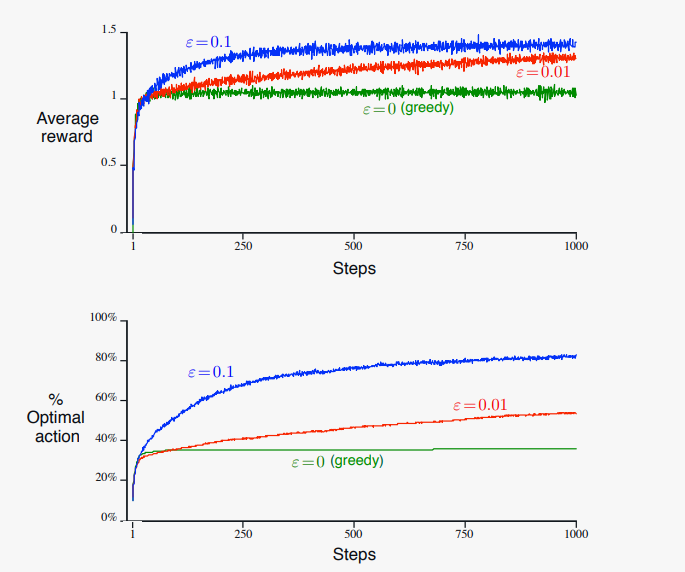
\includegraphics[scale=0.5]{images/textbook-fig-2.2.png}
        \centering
    \end{figure}
\end{homeworkProblem}

    The following are a few ways to balance exploration/exploitation in multi-armed bandits.
    \begin{itemize}
        \item \textbf{Epsilon-greedy}: This is the simplest approach when the bandit has stationary
        probability distributions.
        We choose the greedy action
        with probability $1 - \epsilon$, and we choose a random action with probability $\epsilon$.
        \item \textbf{Optimistic initial values}: We set high initial values for the actions in our
        action-value algorithm, so that we are encouraged to explore more.
        This is because we will always choose the action with the highest estimated reward, so
        with high initial values, the algorithm is more likely to choose various
        actions and therefore explore more.
        \item \textbf{Upper confidence bound (UCB)}: This approach helps choose actions according
        to their potential for actually being optimal (as against a random choice as in the case
        for epsilon-greedy). The UCB action selection uses the following formula (from the textbook):
        \[
            UCB = Q_t(a) + c \sqrt{\frac{\ln t}{N_t(a)}}
        \]
        Where $Q_t(a)$ is the current estimate of the value of action $a$. Also, $c$ is a constant that
        determines the degree of exploration, $t$ is the number of time-steps so far, and $N_t(a)$
        is the number of times that action $a$ has been chosen prior to time-step $t$.
    \end{itemize}

\nobreak\extramarks{Problem 2}{}\nobreak{}

\pagebreak

\nobreak\extramarks{Problem 3}{}\nobreak{}

\begin{homeworkProblem}[Problem 3]
    In the equation,
    \[
        NewEstimate = OldEstimate + StepSize \times [Target - OldEstimate]
    \]
    what is the target?

    \subsection{Answer}

    In general, the target is the presumed desired value of the action-value function that we are
    trying to estimate, or the direction we are trying to move towards. That is why $[Target - Estimate]$
    is known as the \textit{error} in the estimate.\\

    In the specific case of the multi-armed bandit problem, the target is the reward that we received after
    taking the action. With each time step, we attempt to get closer to the target value. For the
    sample-average method used in the multi-armed bandit problem, the equation in the problem takes
    on the following form,
    \[
        Q_{n+1} = Q_n + \frac{1}{n} (R_n - Q_n)
    \]
    where the target is the reward $R_n$ that we received after taking the action.
\end{homeworkProblem}

\pagebreak

\nobreak\extramarks{Problem 4}{}\nobreak{}

\begin{homeworkProblem}[Problem 4]
    What is the purpose of using Upper Confidence Bound (UCB)?

    \subsection{Answer}

    The purpose of using UCB is to provide exploratory behavior balanced with exploitation in a systematic manner.\\

    The UCB formula is as follows,
    \[
        A_t = argmax_a \left[ Q_t(a) + c \sqrt{\frac{\ln t}{N_t(a)}} \right]
    \]
    Here, the square root term is a measure of the uncertainty in the estimate of the current action $a$,
    and $c$ is used to control the confidence level of that uncertainty. The way this square root term
    works is that it increases if the action has not been chosen often (because denominator $N_t(a)$ is
    the number of times the action is chosen), and decreases if the action has
    been chosen often. This means that the action will be chosen more often if it has not been chosen
    much in the past, and less often if it has been chosen a lot in the past.
    The nature of the logarithm term is ideal because, in the beginning it favors exploration overall
    because of high slope,
    but then as all actions are tried, it flattens out and favors exploitation.\\
    
    Therefore, UCB is used to
    approach the true value of an action in a more `systematic' way than epsilon-greedy.

\end{homeworkProblem}

\pagebreak

\nobreak\extramarks{Problem 5}{}\nobreak{}

\begin{homeworkProblem}[Problem 5]
    Why do you think in Gradient Bandit Algorithm, we defined a soft-max distribution to
    choose the actions from, rather than just choosing action?

    \subsection{Answer}
    In the Gradient Bandit Algorithm, we are looking to to create a \textbf{numerical preference}
    for each action. The ideal way to do this is by using the \textit{soft-max distribution},
    or the Gibbs/Boltzmann distribution. This is done by exponentiating the action-value function,
    and then normalizing it. In the form of a formula, this is,
    \[
        \pi_t(a) \doteq \frac{e^{H_t(a)}}{\sum_{b=1}^{k} e^{H_t(b)}}
    \]
    which is the probability of choosing action $a$ at time-step $t$.\\

    The reason we want to create a numerical preference for each action is because we want a snapshot
    in the current time-step of likely we are to select each action. This gives us a high degree
    of predictability in our method. This is a big improvement over the epsilon-greedy method, where
    we have no idea how likely we are to select each action (because with epsilon probability,
    it is random, and just chooses an action).\\
    
\end{homeworkProblem}

\pagebreak

\nobreak\extramarks{Problem 6}{}\nobreak{}

\begin{homeworkProblem}[Problem 6]
    Read the article below and summarize what you learned in a paragraph:

    \href{https://web.archive.org/web/20220122192029/https://www.spotx.tv/resources/blog/developer-blog/introduction-to-multi-armed-bandits-with-applications-in-digital-advertising/}{Introduction to Multi-Armed Bandits with Applications in Digital Advertising}

    \subsection{Answer}

    This article shows how the problem of showing an optimal ad to a user can be modeled as
    a multi-armed bandit problem. Here, an `optimal ad' is one that maximizes the click-through rate (CTR).\\
    
    First, we are shown how we can use the greedy-epsilon method to solve this problem. The
    true probability of a user-click is modeled as 1 trial of a binomial distribution, with the probability
    of success being the CTR, a number chosen arbitrarily. An array of estimated rewards is maintained,
    which the article calls `emperical CTRs'. The greedy-epsilon method is used to choose the ad based
    on an array of weights, where the best ad has a weight of $1 - \epsilon$, and the rest have a weight
    of $\frac{\epsilon}{1 - K}$, where the number of ads is $K$. This experiment set up was run 10,000
    times and the results were plotted in two graphs --- how the emperical CTR changed over the course of
    the runs, and the \% of chosen actions. The analysis of the results showed that the greedy-epsilon
    method found the second most effective ad, and stuck with it for a while, but eventually found
    the most effective ad.\\

    The second method of modeling the problem we are shown is the Thompson sampling method. Here,
    Bayesian beliefs are used to model the probability of a user clicking on an ad. Therefore, instead
    of using an array of weights like in the greedy-epsilon method, we use a beta distribution to
    choose the ad. As more clicks are recorded, the alpha and beta arrays for each ad is updated.
    If the chosen ad was clicked, then we update the alpha array, and if it was not clicked, we update
    the beta array. The results of this experiment were also plotted in the same way as the greedy-epsilon
    approach. The analysis of the results showed that the Thompson sampling method found the most effective
    ad much faster than the greedy-epsilon method.\\

    In the final part of the article, a concept of comparing the two methods is introduced: \textit{regret}.
    Regret is defined as the difference between the reward of the optimal action and the reward of the
    chosen action. Via a definitive plot, the
    regret for the greedy-epsilon method was found to be much higher than the regret
    for the Thompson sampling method. Therefore, the Thompson sampling method is the better method
    for this problem.

\end{homeworkProblem}

\end{document}